Until Edwin Hubble's measurement of the distances to M31 and M33 using Cepheid variable stars in the early twentieth century (\citealt{Hubble_1925}), many astronomers believed that the Milky Way encompassed all matter in the Universe. Observational data of the time meant that all extragalactic sources, appearing as small, hazy patches of light in the sky, were indistinguishable from clusters of stars, gas and dust that are part of our own Galaxy. Objects that were not immediately identifiable as stars were given the name \textit{nebulae} (Latin for 'clouds') which included Galactic sources as well as hitherto unknown extragalactic sources such as the \textit{Andromeda Nebula}. The consequence of this confusion is still evident in astronomy today in the naming convention used for certain catalogues, such as the Messier Catalogue, which consists of star clusters, nebulae and supernova remnants within the Galaxy as well as other galaxies, including \textit{Andromeda} (M31).

Since this initial discovery, the number of catalogued galaxies in the observable Universe has been ever increasing. Thanks to the finite speed of light, the history of star formation in the Universe can be observed directly from the light of distant galaxies as we look back time. Deep observations allow us to explore the evolution of galaxies from the early Universe to the galaxies we observe around us today. In particular, the deepest fields give astronomers the opportunity to look back at a time when galaxies were first forming. In 1995, the \textit{Hubble Space Telescope} was directed toward a small patch of sky covering only 1/30th the diameter of the full moon, for 10 consecutive days in order to capture a "keyhole" view of the Universe. The resulting image, known as the Hubble Deep Field (HDF, Figure \ref{fig:hubble_deep_field}), revealed a spectrum of almost $3,000$ galaxies with various morphologies, sizes and colours, despite the narrow field appearing to have nothing remarkable to the naked eye. The isotropic distribution of galaxies in all lines of sight suggests that this small sample of the total sky represents a typical distribution of galaxies from the early Universe to today. In this image there are particularly dim, red galaxies that may have formed within the first billion years after the Big Bang. At these high redshifts the distribution of objects is skewed towards asymmetric and irregular galaxies (\citealt{Abraham_1996}), whereas in the foreground we observe a plethora of spiral- and elliptical-shaped galaxies. The vast quantities of galaxies in the HDF at different stages in their evolution raises important questions about how galaxies evolve from the young Universe to today, especially given that such an image will naturally be a "family photograph" of galaxies with some of their own ancestors at earlier times. We raise some important questions about the formation and evolution of galaxies prompted by this deep image: why are there different types of galaxies? do the properties of their stellar and gaseous contents differ? how did these galaxies form? do they represent distinct populations or are we witnessing a variety of snapshots in the evolution of a typical galaxy? In this thesis {\color{red}[...]}.

\begin{figure}
    \centering
	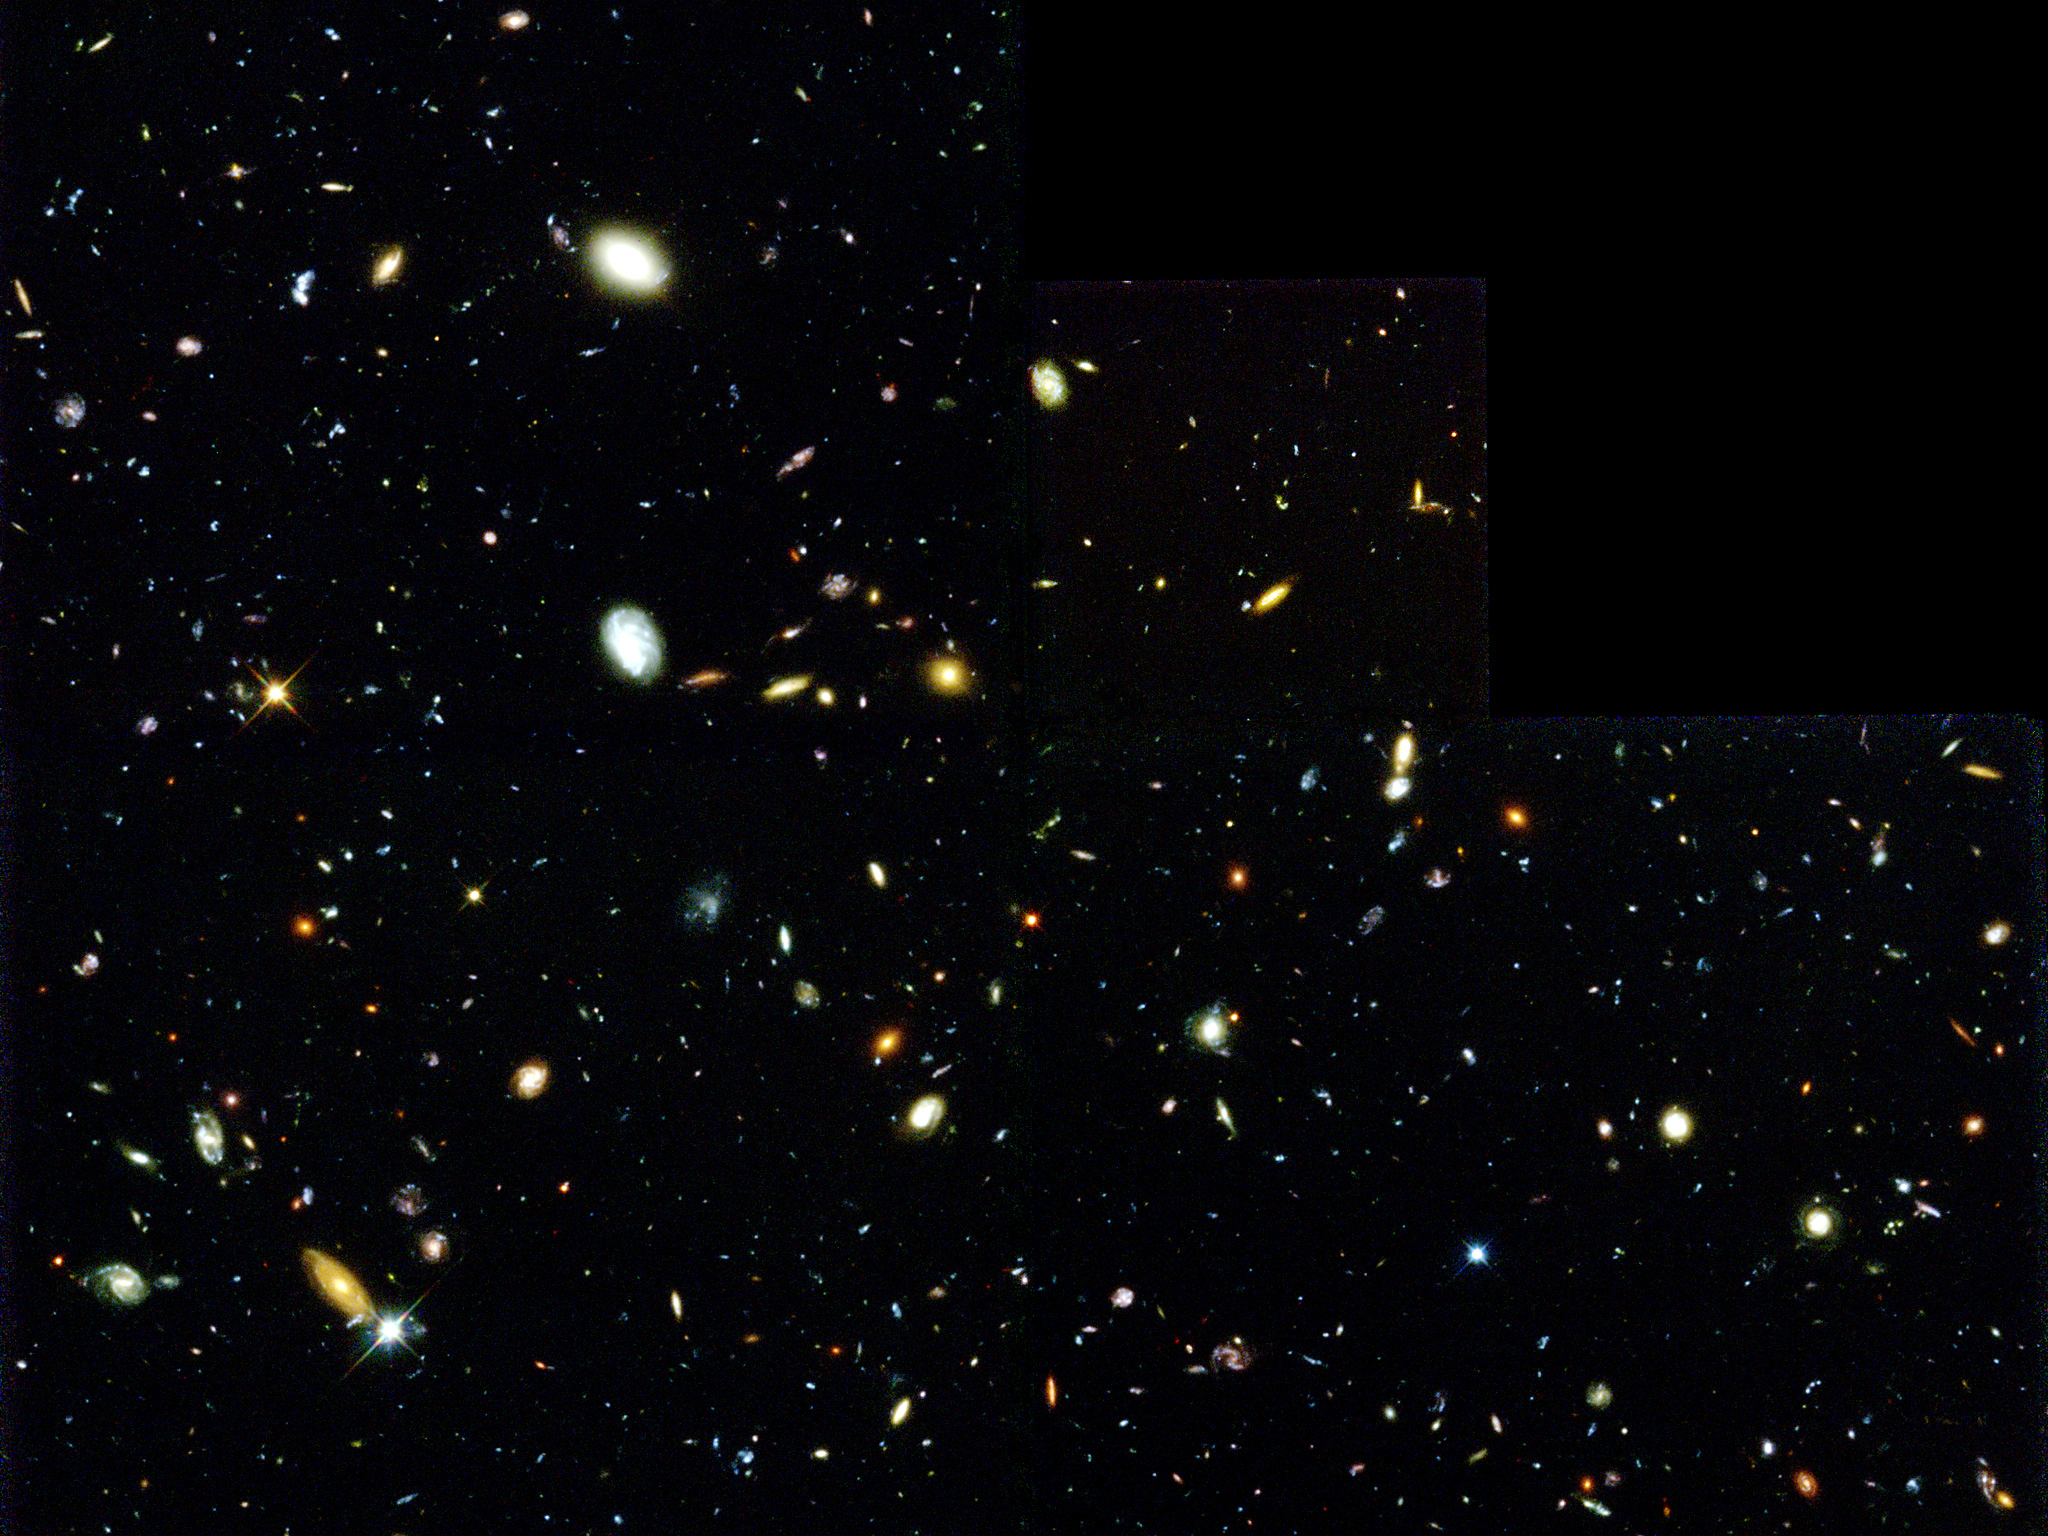
\includegraphics[width=0.9\columnwidth]{Figures/hubble_deep_field.jpeg}
	\caption{The Hubble Deep Field as captured by the Wide Field and Planetary Camera 2 onboard the \textit{Hubble Space Telescope} in 1995.}
	\label{fig:hubble_deep_field}
\end{figure}

\section{Galaxy Formation and Evolution}

To answer our questions on the evolution of galaxies, we must first make some inferences about the {\color{red}[...]} of the Universe. Our understanding of the cosmic history of galaxies is dependent on our choice of cosmology, which is widely accepted to be in the form of the $\Lambda$-CDM model (\citealt{Peebles_1980}). In the $\Lambda$-CDM model, Cold Dark Matter, matter of unknown origin, dominates over ordinary baryonic matter; and with dark energy, constitute a combined $\sim 95\%$ of the total cosmic energy budget (\citealt{Fukugita_2004}). The presence of dark matter is only evident in its gravitational interactions with other matter, but its origin is unknown as it does not interact with nor emit any electromagnetic radiation. The dark energy in the Universe is parameterized in the form of the cosmological constant, $\Lambda$, which is required to explain the accelerating expansion of the Universe. In this model, galaxy formation is seeded by small quantum fluctuations in the density of the early Universe, which grow with inflation to form small overdensities that later become the sites of dark matter halos by gravitationally attracting nearby dark matter. The first galaxies formed from these originally minute overdensities in density, which later merge due to an increase in collisions in a smaller Universe, to form ever larger galaxies. This model of galaxy formation is called a 'hierarchical' model, where galaxies in the early Universe are expected to be smaller and formed their mass more quickly than massive galaxies at later times that formed much of their stellar mass from previous mergers. As we shall show in Chapter \ref{chapter:Radio_Identifications}, this model of evolution may not explain the stellar build up of all galaxies.

\subsection{Classification of Galaxies}

The first step in understanding galaxy evolution by observing how galaxies have changed as we look back in time, is to classify galaxies according to their observable properties. Generally, galaxies can be classified into two broad groups based on their morphology: spirals and ellipticals. This dichotomy prompted the first classification scheme by Edwin Hubble (Figure \ref{fig:hubble_tuning_fork}; \citealt{Hubble_1936}), the \textit{Tuning Fork}, which shows ellitpical galaxies along the "handle", becoming more oblate towards the spiral galaxies. The spiral galaxies themselves are split into two categories forming the two "prongs", depending on the presence of a bar at the centre. At the join of the two, classified on the \textit{Tuning Fork} as S0, is where we might locate \textit{lenticular galaxies}, that are recognized by their large disks, like spirals, but without the presence of arms. In the rest of this Thesis we shall predominantly be referring to elliptical galaxies at \textit{early-type galaxies} (ETGs) and spiral-like galaxies as \textit{late-type galaxies} (LTGs), as is convention. Despite their names, the two do not represent a former and latter evolutionary stage of a typical galaxy, and is rather a misnomer. A minority of galaxies do not conform to this dichotomous image and are typically grouped together as \textit{irregular galaxies}.

\begin{figure}
    \centering
	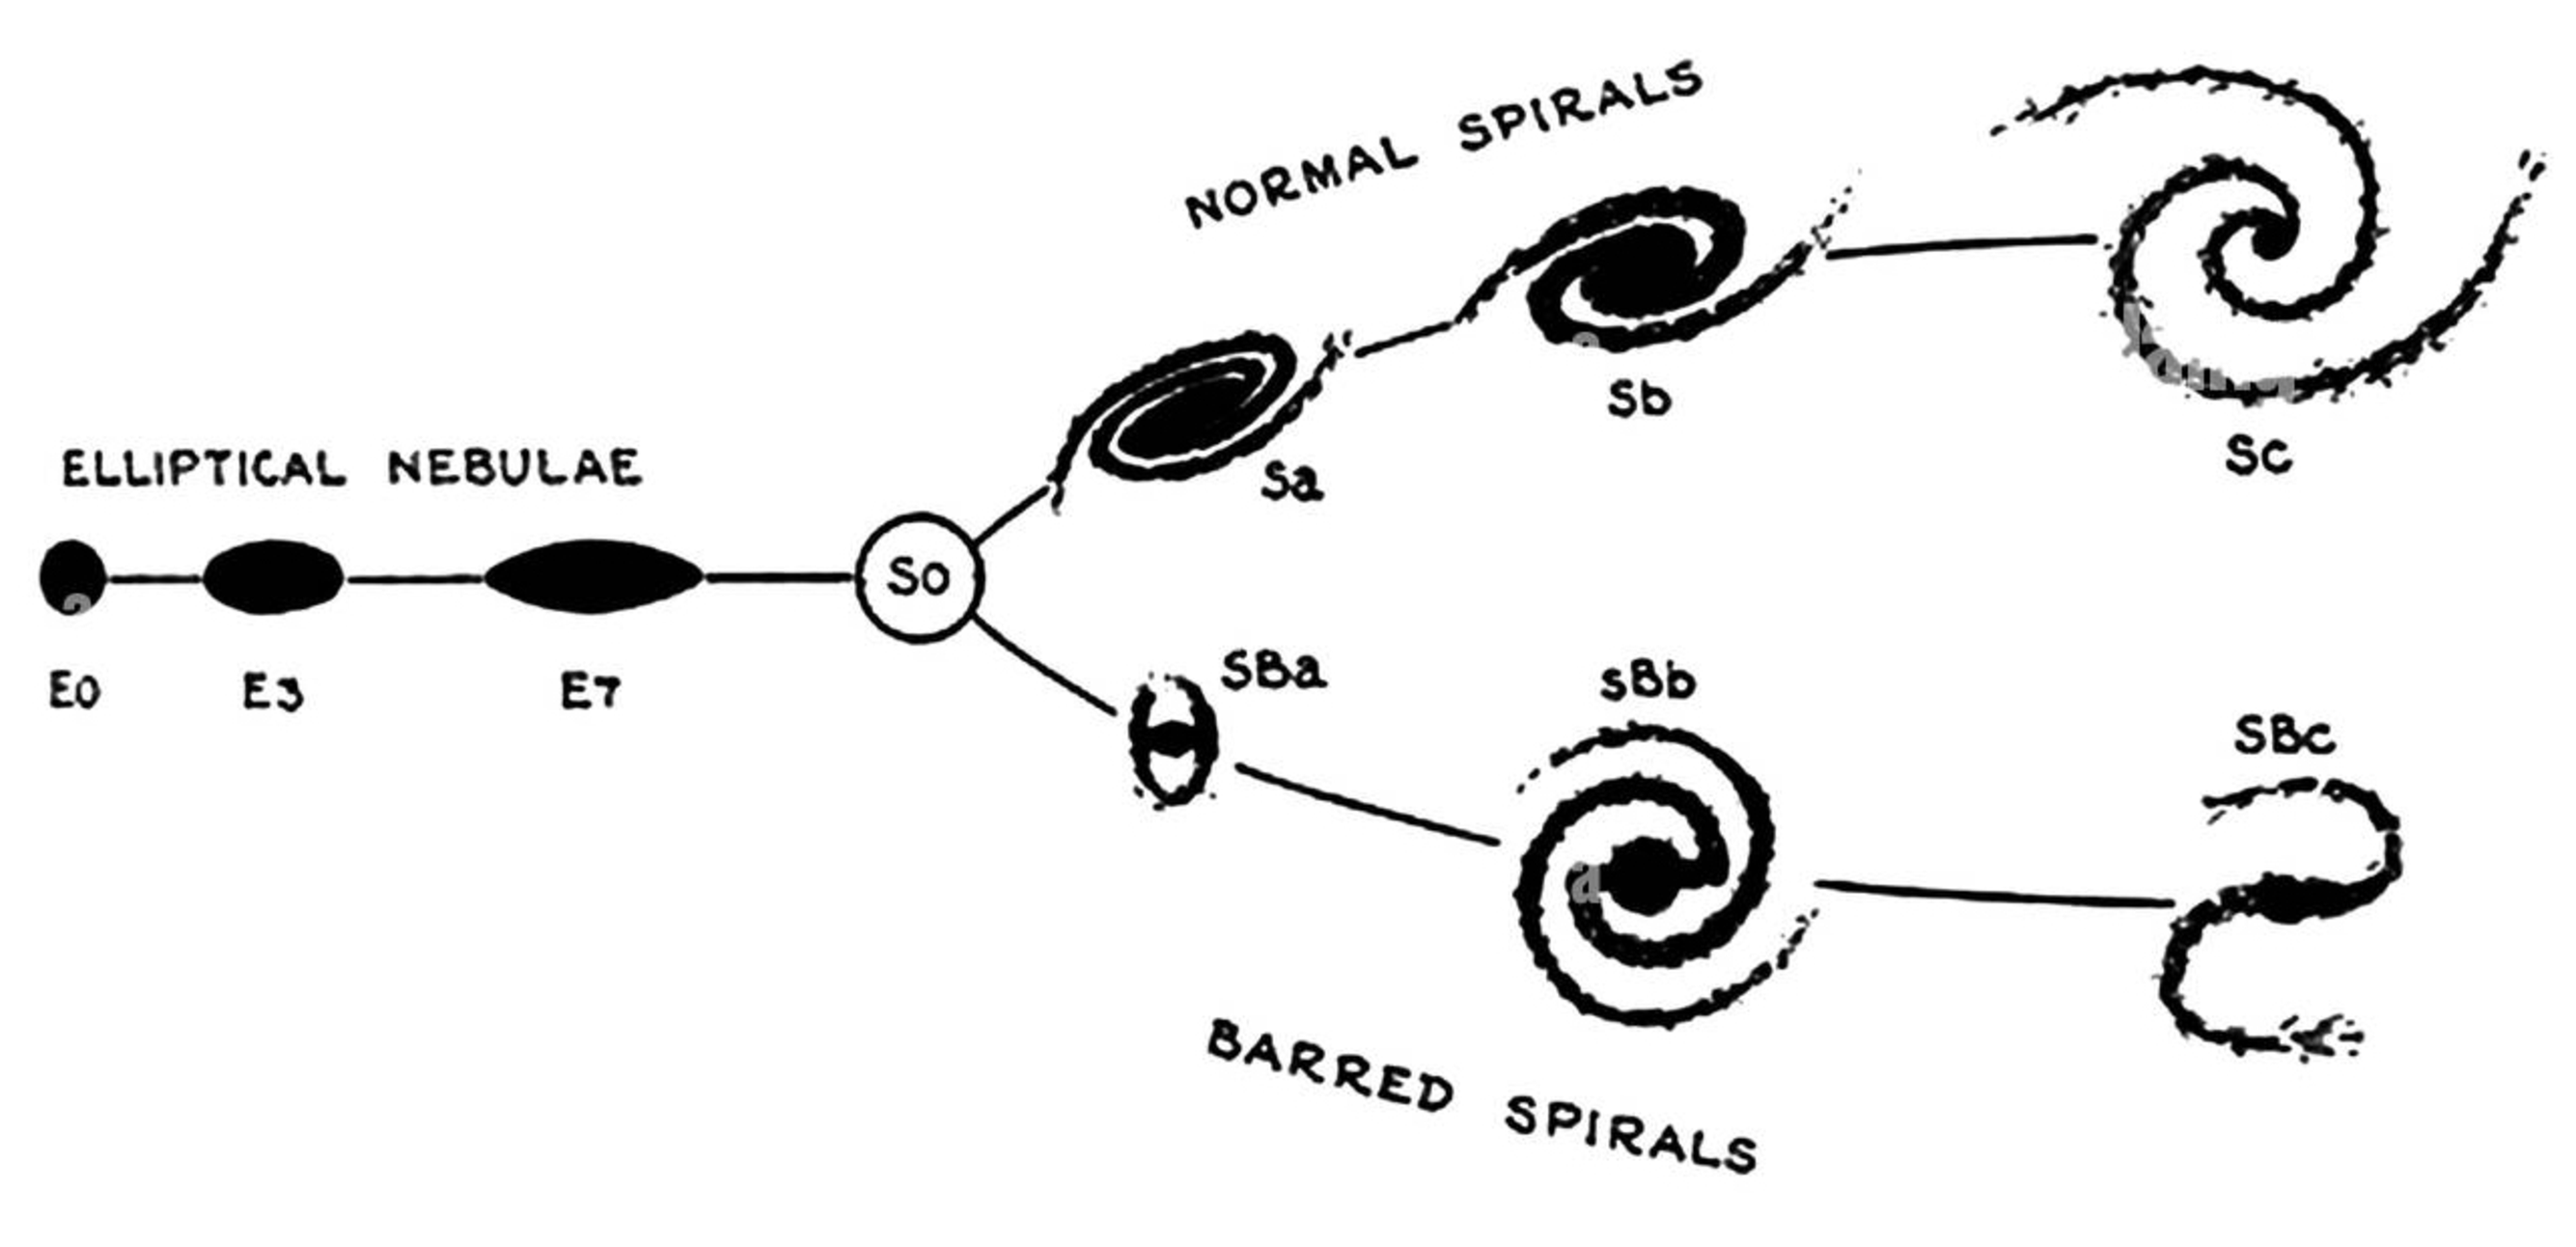
\includegraphics[width=0.9\columnwidth]{Figures/hubble_tuning_fork}
	\caption{The \textit{Hubble Tuning Fork}, or the \textit{Sequence of Nebular Types} as named in \citealt{Hubble_1936}, showing spiral galaxies along the prongs of the tuning fork and elliptical galaxies along the handle. The two prongs separate those spiral galaxies with barred central bulges from those that do not. Lenticular galaxies can be found at the join of the handle to the prongs. From left to right, the elliptical galaxies become more oblate and the spiral galaxies have spiral arms that become less tightly wound around the central bulge.}
	\label{fig:hubble_tuning_fork}
\end{figure}

Beyond their shape, the two broad groups, ETGs and LTGs, have a number of physical characteristics that are common to galaxies of the same class. First, the stellar populations of ETGs and LTGs are different. ETGs are dominated by old stellar populations that appear red in colour because they contain longer-lived, low mass stars, whereas LTGs typically have younger stellar populations of massive, but very short-lived stars.

ETGs are considered to be some of the most massive, luminous galaxies (due to having vast quantities of old stars) observed in the local Universe (\citealt{Bernardi_2003}; \citealt{Kelvin_2014}; \citealt{Moffett_2016}). Their stellar content is often centrally distributed, with the density of stars decreasing to the outskirts of the galaxy. In this central bulge of stars is where most of the interstellar medium (ISM) is located, though it is not expected to be substantial, and the limited amount of gas prohibits new star formation. In a hierarchical view of star formation, such ellipticals are formed from a series of major and minor mergers that consume the gas in the galaxy, leading to the quiescent systems observed today (\citealt{Toomre_1972}). In contrast, LTGs have dusty spiral arms with sites of active star formation, with older stars mainly located within the central bulge. While ETGs are largely devoid of gas, LTGs have a rich ISM that continues to fuel star formation, creating new stars at typical rates of several stars per year (\citealt{Kennicutt_1983}; \citealt{Gao_2004}). Our own Milky Way is an SBc spiral galaxy (\citealt{Gerhard_2002}) with active star formation at a rate of $\sim 2\,M_\odot$yr$^{-1}$ (\citealt{Noriega-Crespo_2013}; \citealt{Licquia_2015}; \citealt{Elia_2022} and references therein).

\subsection{The Star Forming Main Sequence}

A natural diagram to illustrate the difference in colour of ETGs and LTGs is to show the colours of optically-selected galaxies against their absolute magnitude. Galaxies discovered in optical surveys readily form two distinct regions: a \textit{red sequence} and a \textit{blue cloud}, with a sparsely populated region in between, the \textit{green valley}. Due to their optical colours, the red sequence is dominated by ETGs and the blue cloud dominated by LTGs. Moving away from observed quantities to intrinsic quantities, we note that the colour is a strong indicator of the star formation rate (SFR) in a galaxy and that absolute magnitude is approximately proportional to the size of the stellar population, and thus the stellar mass, $M_*$. In this formalism, the blue galaxies form a tight correlation known as the \textit{Main Sequence} (MS) or \textit{Star Forming Main Sequence}, while the red sequence occupies a \textit{passive cloud} (or "red and dead" or "quiescent") region that lies below the MS at lower star formation rates (\citealt{Noeske_2007}; \citealt{Daddi_2007}; \citealt{Elbaz_2007}; \citealt{Rodighiero_2011}). Figure \ref{fig:star_forming_main_sequence} shows the main sequence and passive clouds (grey contours) that form from the optically-selected Sloan Digital Sky Survey (SDSS; \citealt{York_2000}). \citealt{Saintonge_2017} present the \textit{Extended CO Legacy Database for GASS}, xCOLD GASS, a mass-selected sample from SDSS that have molecular gas mass estimates, which are plotted in colour in Figure \ref{fig:star_forming_main_sequence}. The molecular gas mass fraction, $f_{\textrm{H}_2} \equiv M_{\textrm{H}_2}/M_*$, clearly declines towards the passive cloud, showing the depleted ISM in ETGs.

{\color{red}Perhaps add a paragraph on the stellar-mass growth sequence, as illustrated by Figure 12 of Graham+2023}

\begin{figure}
    \centering
	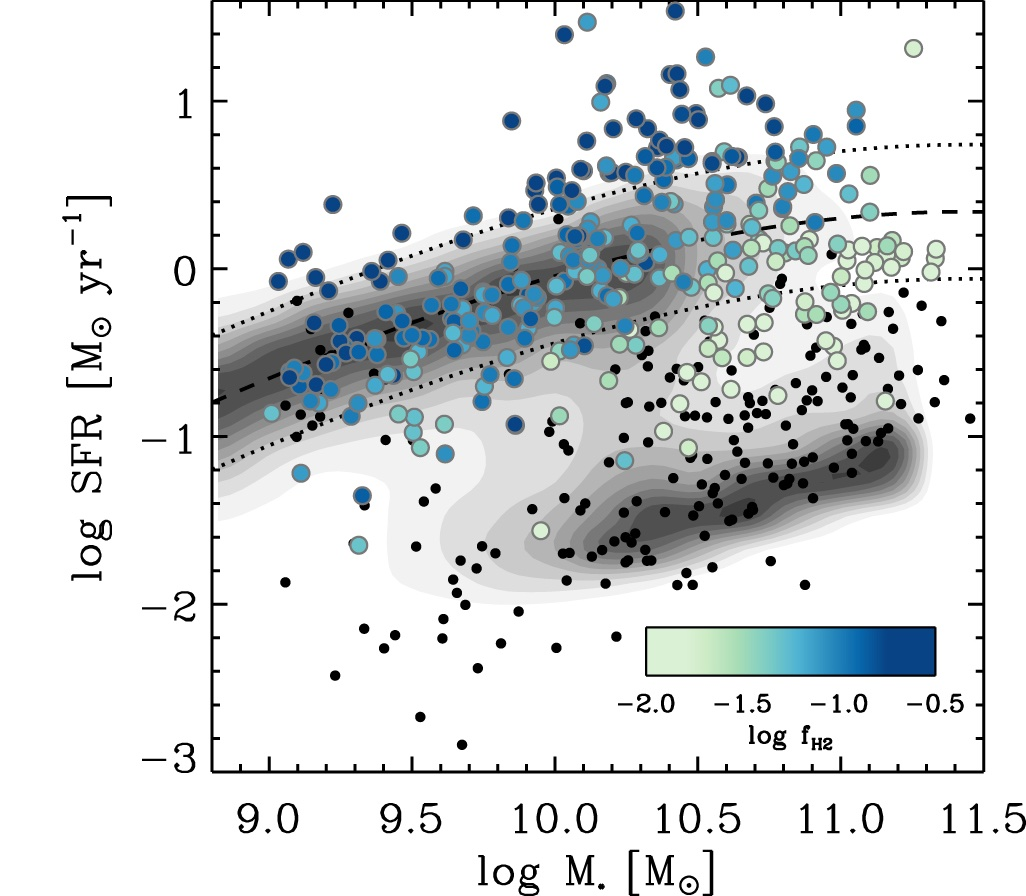
\includegraphics[width=0.75\columnwidth]{Figures/saintonge_ms.jpg}
	\caption{The distribution of SDSS galaxies in the SFR-$M_*$ plane (grey contours) from \citealt{Saintonge_2017} (Figure 7). The dashed line represents the location of the main sequence, while the dotted lines represent $\pm0.4\,$dex scatter around this relation. The coloured points show the distribution of galaxies from xCOLD GASS, coloured according to their molecular gas mass fraction.}
	\label{fig:star_forming_main_sequence}
\end{figure}

It is predicted that the vast majority, approximately $90\%$, of all cosmic star formation between redshifts $0$ and $2.5$ occurs in galaxies that reside on the MS, however, an important contribution also comes from galaxies that sit substantially above the relation. These galaxies, undergoing high levels of star formation for a short period of time, are collectively referred to as \textit{starburst galaxies} (e.g. \citealt{Muxlow_2006}; \citealt{Rinaldi_2022}). Starbursts form a small minority of galaxies, approximately $2\%$ of star forming galaxies depending on the exact definition of a starburst, but contribute $\sim 10\%$ of the cosmic star formation rate density (SFRD) at $z \sim 2$ (\citealt{Rodighiero_2011}), corresponding to the time in cosmic history when star formation was at its peak (see Section \ref{sec:cosmic_star_formation_history}).

Given that galaxies in the passive cloud have large stellar masses, they must have been at some point among the actively star forming galaxies, and then some process quench them of their star formation leading them to the passive cloud. The prevailing interpretation of the SFR-$M_*$ diagram is that a typical galaxy evolves along the sequence, gaining stellar mass, increasing their star formation rate accordingly and depleting the gas available for star formation in the process. At some point, the galaxy stops forming stars entirely, and falls off the main sequence. The valley between the MS and the passive cloud, a result of a dearth of galaxies in this regime, suggests that the quenching process that turns off the star formation in the galaxy is fast. This image of galaxy evolution, however, is not without scepticism. Recent studies (e.g. \citealt{Eales_2018}; \citealt{Bremer_2018}; \citealt{Phillipps_2019}) have suggested that the bimodal distribution of star forming and passive galaxies may be a reflection of selection effects in optical surveys, prompting attempts to define the whole population of galaxies using a probability distribution with only one maximum (e.g. \citealt{Corcho-Caballero_2020}). {\color{red}Explain the evidence for an apparent bimodality (Read abstracts of three papers above - that is all that is needed.)}

Whether there are two distinct classes or whether the transition between morphological types and physical properties is gradual, some physical process must be coverting a star forming galaxy on the MS to one that is passive, quenching it of star formation. There are many possibilities that have been proposed as the cause of quenching, and it is likely that all are important in different scenarios. These processes include stellar feedback and winds from supernovae removing the gas from a galaxy (\citealt{Hayward_2017}); gas expulsion by active galactic nuclei, AGN (\citealt{Springel_2005}; \citealt{Croton_2006}; \citealt{Cicone_2014}; \citealt{Harrison_2017}); the formation of a galactic bar or central bulge (\citealt{Bournaud_2007}; \citealt{Martig_2009}) which relocates the gas to the galactic center and reduces the star formation in the disk, as well as a range of environmental processes such as galaxy merging (\citealt{Lavery_1994}; \citealt{Weigel_2017}) which ignites a starbursting phase that rapidly consumes the gas; ram-pressure stripping, the loss of gas as the galaxy passes through the intra-cluster medium (\citealt{Gunn_1972}; \citealt{Boselli_2006}; \citealt{Domainko_2006}; \citealt{Boselli_2014}), and quenching mechanisms that result from being in high density environments such as galaxy clusters, like galaxy harassment and strangulation (\citealt{Moore_1996}; \citealt{Moore_1998}; \citealt{Bekki_2002}).

\subsection{Cosmic Star Formation History}
\label{sec:cosmic_star_formation_history}

We have seen that the star formation rates of galaxies is intrinsically linked to its evolutionary stage, and thus it would be unsurprising to identify an evolution in the integrated SFRs of galaxies with cosmic time. By measuring the star formation of many galaxies at different epochs, we can build a picture of the star formation density in the Universe. The cosmic history of star formation is one of the fundamental observables of astronomy, giving us an insight into the timeline for which gas forms into stars, heavy elements are produced (elements heavier than the primordial Hydrogen and Helium are produced in stars), and dust is formed (as dust is a natural byproduct of star formation, see Section {\color{red}X}).

The cosmic star formation rate density (SFRD {\color{red}Repeated}) in the Universe can be estimated in two ways. The most straightforward way to estimate the star formation rate is to measure the amount of starlight we observe from tracers of recent star formation in galaxies. In this sense, the SFR indicator should be sensitive to the short-lived massive stars at each point in cosmic history, and thus the UV and optical stellar light is often used. Second, we note that approximately half of all optical and UV light from stars ever emitted in the Universe has been absorbed by dust and re-emitted at far-infrared (FIR) and sub-millimeter (sub-mm) wavelengths (\citealt{Puget_1996}; \citealt{Fixsen_1998}; \citealt{Dole_2006}; \citealt{Driver_2016}). This means that a significant contribution to the SFRD must also be measured from far-IR/sub-mm indicators of star formation that probe the stellar light reprocessed by dust.

Figure \ref{fig:cosmic_sfrd} shows that the dust obscured and unobscured measures of the SFRD have peaks at $z\sim2$ (when the Universe was roughly 3 billion years old), followed by a slow decline to the present day. The short period corresponding to the peak of star formation is often referred to as \textit{cosmic noon}. In the (approximate) 3.5\,Gyr between $z\sim3$ and $z\sim1$, spanning cosmic noon, up to half of the stellar mass we observe today was formed (\citealt{Forster-Schreiber_2020}). The galaxies that are identified at these redshifts are ideal targets for tracing the formational epoch of the massive LTGs and ETGs seen in the local Universe.

\begin{figure}
    \centering
	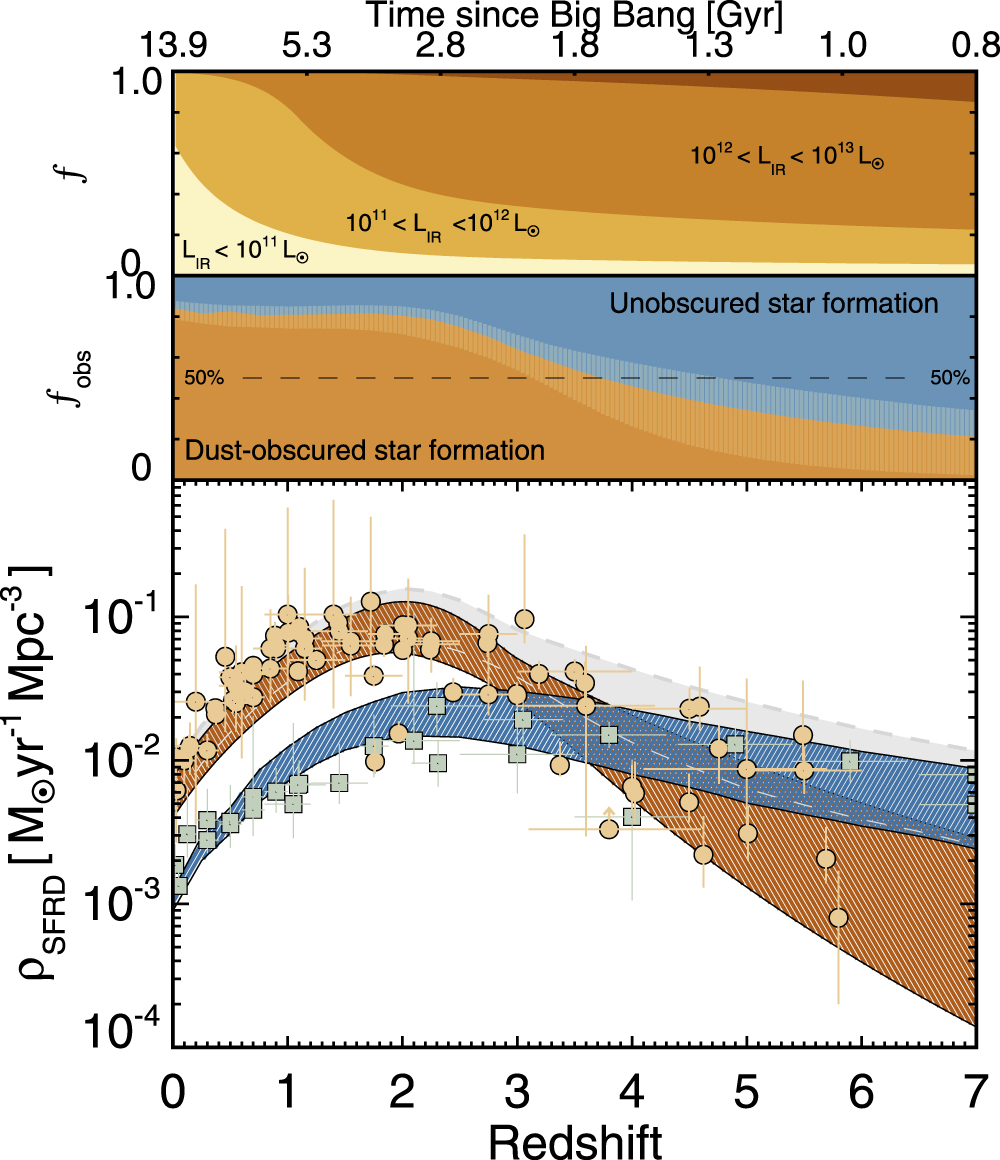
\includegraphics[width=0.75\columnwidth]{Figures/cosmic_sfrd.jpeg}
	\caption{The cosmic star formation history from \citealt{Zavala_2021}. The contributions to the total star formation rate density (grey) from dust obscured IR/sub-mm surveys and from unobscured UV/optical surveys are shown in orange and blue, respectively. The top panel shows the contribution from galaxies with different IR luminosities to the dust obscured SFRD. The classes shown are $L_\textrm{IR} < 10^{11}\,L_\odot$, $10^{11} < L_\textrm{IR} [L_\odot] < 10^{12}$ (LIRGs) and $10^{12} < L_\textrm{IR} [L_\odot] < 10^{13}$ (ULIRGs). The middle panel represents the fraction of SFRD that is dust obscured.}
	\label{fig:cosmic_sfrd}
\end{figure}

{\color{red}Dust contribution}
